% generated by make_figs.mjs
\resizebox{\columnwidth}{!}{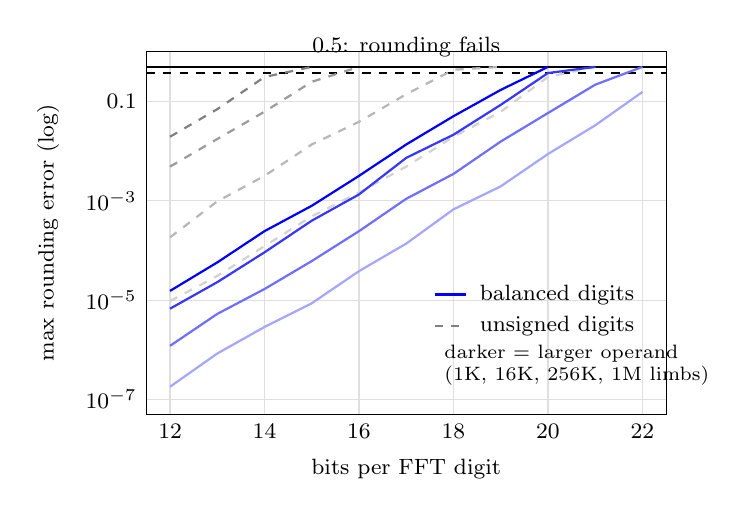
\begin{tikzpicture}[font=\footnotesize]
\draw[gray!25] (0,0.189) -- (6.6,0.189); \node[left] at (0,0.189) {$10^{-7}$};
\draw[gray!25] (0,1.449) -- (6.6,1.449); \node[left] at (0,1.449) {$10^{-5}$};
\draw[gray!25] (0,2.710) -- (6.6,2.710); \node[left] at (0,2.710) {$10^{-3}$};
\draw[gray!25] (0,3.970) -- (6.6,3.970); \node[left] at (0,3.970) {$0.1$};
\draw[gray!25] (0.300,0) -- (0.300,4.6); \node[below] at (0.300,0) {12};
\draw[gray!25] (1.500,0) -- (1.500,4.6); \node[below] at (1.500,0) {14};
\draw[gray!25] (2.700,0) -- (2.700,4.6); \node[below] at (2.700,0) {16};
\draw[gray!25] (3.900,0) -- (3.900,4.6); \node[below] at (3.900,0) {18};
\draw[gray!25] (5.100,0) -- (5.100,4.6); \node[below] at (5.100,0) {20};
\draw[gray!25] (6.300,0) -- (6.300,4.6); \node[below] at (6.300,0) {22};
\draw (0,0) rectangle (6.6,4.6);
\node at (3.3,-0.7) {bits per FFT digit};
\node[rotate=90] at (-1.25,2.3) {max rounding error (log)};
\draw[black,thick] (0,4.410) -- (6.6,4.410) node[pos=0.5,above] {0.5: rounding fails};
\draw[black,dashed] (0,4.332) -- (6.6,4.332);
\draw[blue!35,thick] plot coordinates {(0.300,0.348) (0.900,0.770) (1.500,1.107) (2.100,1.408) (2.700,1.816) (3.300,2.166) (3.900,2.601) (4.500,2.893) (5.100,3.304) (5.700,3.668) (6.300,4.092)};
\draw[gray!35,thick,dashed] plot coordinates {(0.300,1.436) (0.900,1.755) (1.500,2.134) (2.100,2.513) (2.700,2.814) (3.300,3.144) (3.900,3.523) (4.500,3.841) (5.100,4.282) (5.700,4.410)};
\draw[blue!56.66666666666667,thick] plot coordinates {(0.300,0.867) (0.900,1.273) (1.500,1.589) (2.100,1.944) (2.700,2.324) (3.300,2.735) (3.900,3.051) (4.500,3.462) (5.100,3.824) (5.700,4.184) (6.300,4.410)};
\draw[gray!56.66666666666667,thick,dashed] plot coordinates {(0.300,2.245) (0.900,2.703) (1.500,3.026) (2.100,3.425) (2.700,3.713) (3.300,4.063) (3.900,4.374) (4.500,4.410)};
\draw[blue!78.33333333333334,thick] plot coordinates {(0.300,1.339) (0.900,1.676) (1.500,2.055) (2.100,2.457) (2.700,2.790) (3.300,3.255) (3.900,3.549) (4.500,3.928) (5.100,4.332) (5.700,4.410)};
\draw[gray!78.33333333333334,thick,dashed] plot coordinates {(0.300,3.144) (0.900,3.494) (1.500,3.841) (2.100,4.221) (2.700,4.410)};
\draw[blue!100,thick] plot coordinates {(0.300,1.565) (0.900,1.927) (1.500,2.324) (2.100,2.646) (2.700,3.026) (3.300,3.425) (3.900,3.784) (4.500,4.118) (5.100,4.410)};
\draw[gray!100,thick,dashed] plot coordinates {(0.300,3.523) (0.900,3.873) (1.500,4.282) (2.100,4.410)};
\draw[blue,thick] (3.660,1.520) -- +(0.4,0);
\node[anchor=west] at (4.110,1.520) {balanced digits};
\draw[gray,thick,dashed] (3.660,1.120) -- +(0.4,0);
\node[anchor=west] at (4.110,1.120) {unsigned digits};
\node[anchor=west,font=\scriptsize,align=left] at (3.660,0.620) {darker = larger operand\\(1K, 16K, 256K, 1M limbs)};
\end{tikzpicture}}
